\chapter{Related Work}
%----------------------------------------------------

\section{Aggregated overview about paper describing MR learning systems}
nur gedankenstütze: "In order to create a study design to evaluate the perspective and learning we here take a look on how other researchers conducted their studies"

\subsection{Method}
Jacky Chan et al. \todo created a VR dance training system using an optical motion capturing system to compare the movements performed by the student with movements from the avatar. These movements are presented to the student as a 3D rendering on large screen. The movements of the students are visualised on the same screen as a coloured stick figure. The student mimics these movements and gets instant feedback as well as a feedback as a summary.

In contrast, Onebody by Hoang et al. \todo use a VR headset for a first person remote posture guidance system. 

\subsection{Tasks}
In Chan et al. \todo the dance student is presented a virtual avatar performing dance moves of A-go-go or Hip-Hop style. The avatars movement is based on the motion capturing data of a professional dancer. Onebody \todo is not only restricted to dance moves but also include other posture based sports or physical activities like Yoga or Mixed Martial Arts.

Onebody \todo uses a number of martial arts postures or stances.

\subsection{Measures and variables}
Jacky Chan et al. \todo defined 19 body parts that are considered in the measure of the performance of the dancing student. They name three features to compare the difference between two motions common: joint position, joint velocity and joint angle. Chan investigated which of these features suits most to judge the two dancing motions. The outcome of this investigation names the joint position to have the highest discriminative power. Hence, the joint position suits them best for their evaluation, Chan et al. calculate a score of the position error for each of the defined body parts, as well as an overall score. 

Onebody \todo uses skeletal of the instructor and the student
"Posture accuracy is determined by the extend to which the student can replicate the final posture as instructed and demonstrated as by the instructor." Independent variable: mothods for posture training. dependent variables: performance factors of posture accuracy, completion time, subjective instructor rating, users preference.


\section{Detailed description of 6-10 papers incl. Table}
%hier werden die paper detailiert vorgestellt von denen ich dann meine tasks, measures, methode und variablen ableite. am ende zusammenfassung in einer tabelle
\subsection{Onebody: Remote Posture Guidance System using First Person View in Virtual Environment}
\begin{itemize}
	\item[Hardware:] Kinect, Oculus Rift
	\item[Task:] sports, dance, martial arts, yoga
	\item[Perspectives:] First Person of the teacher
	\item[Measures:] Position - skeletal matching with 5cm threshold
	\item[investigation:] comparing different remote guidance systems: onebody, pre recorded video, video conference, VR third person
\end{itemize}
Onebody by Hoang et al. \todo is a VR system for remote posture guidance. Onebody is designed for sports or physical activity training like yoga, dance or martial arts. The student and the teacher are both tracked by skeletal tracking. The visualisation of this tracking are shown via a VR headset, allowing the student to follow the instruction of the teacher in first person view of the teacher - which means the student "stands inside the body of the teacher". Both, the student and the teacher are visualised by stick figures. The teachers avatar is red, the students blue and matching joints are green like shown in figure \ref{fig:ob1} left. Figure \ref{fig:ob1} right shows the scene from the first person perspective.
\begin{figure}
	\centering
	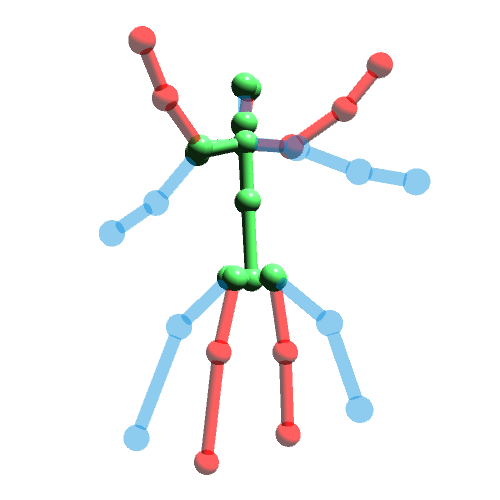
\includegraphics[width=0.225\textwidth]{img/onebody1.png}
	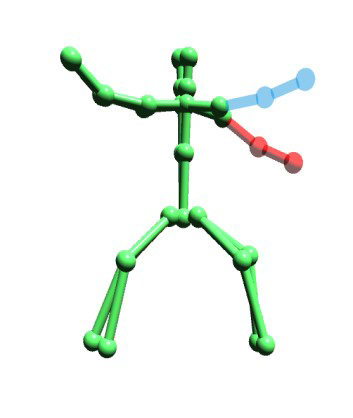
\includegraphics[width=0.225\textwidth]{img/onebody2.png}
	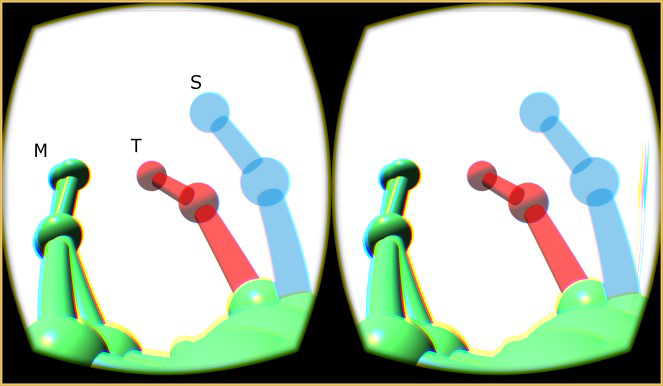
\includegraphics[width=0.45\textwidth]{img/onebody3.png}
	\caption{Left: student avatar (blue) and teacher avatar (red). Green limbs are matching limbs. Right: students view on the scene.\todo}
	\label{fig:ob1}
\end{figure}
When the teacher moves his limbs, the student can see the movement emerging from himself. Now the student can move his own limbs to mimic the movement till the teachers posture is matched. The teacher sees the students limbs likewise allowing him to give instant feedback to the student. Thus, "Onebody provides a medium to deliver body movement instructions for non-collocated instructor and learner." \todo. The visualisations are attached to the hip but keeps the mapping between the user and corresponding avatar. To overcome different body sizes, the avatars are normalised and scaled to the size of the person seeing the avatars.\\
For transfering data, both the teacher and the student are clients in a server-client system. The clients are sending the their tracking data to the server which is broadcasting it to the clients. The comparison of the limbs for colour coding is performed on the client side. The matching of the limbs is calculated by the position of the single limbs (see equation \eqref{eq:constanterror}) with a threshold of 5cm to reduce jitter and tracking errors. The feedback with colour codes is provided in realtime.

\section{Research Gap}

\section{Conclusion (and research questions/hypothesises?)}
hier wird zusammengefasst was ich abgeleitet habe und direkt in das studien design einfließt. danach folgen die genauen RQ und hypothesen.

\begin{comment}
\begin{itemize}
	\item task is xyz because of abc
	\item measures are xyz because of abc
	\item variables are...
\end{itemize}


\section{MR learning systems}
\begin{itemize}
	\item one body:
	\item vr dance trainer:
	\item you move:
	\item training archived physical skills:
	\item
	\item teaching traditional dance using e-learning tools, bakogianni
\end{itemize}

%----------------------------------------------------
\section{Ego/exo perspective work - if exists}
\begin{itemize}
	\item training archived physical skill: seamless change from first to third person
\end{itemize}
%----------------------------------------------------
\section{variables}
\begin{itemize}
	\item independent/dependent variables
	\item measures
	\item task: reuse or adapt existing task
\end{itemize}
%----------------------------------------------------
\subsection{Task}
\begin{itemize}
	\item Onebody: 16 artificial postures not from but like: tai chi, matial arts
	\item VR Dance Trainer: dance movements, 15 min for each move
	\item you move: various movements to perform. using a whip, baseball, boxing, ballet, dance moves
	\item training archived physical skills IVE: physical skills in sport activities, especially baseball pitching
\end{itemize}
%----------------------------------------------------
\subsection{Measures}
\begin{itemize}
	\item scientific work, how to measure movements: hachimura et al, yoshimura et al, qian et al, kwon et al, all use joint angles,  (mentioned in: vr dance trainer)
	\item onebody: skeletal tracking, how much percent do the postures match? 3d positions of limbs measured: wrist, elbow, shoulder, hip knee ankle. so angle between bones is the main measure for accuracy. additionally a subjective instructor score was recorded. And, completion time, topped by 2 min.
	\item VR Dance trainer: there are 3 common features for measuring hte difference between movements: joint position, velocity, angle. they tested which feature descibes movements best: joint position. base line vs post training movements are compared.
	\item you move: in each keyframe, score based on the joint with the maximum error, measured in euclidean distance. but only "important joints" are measured. timing errors: 0.5s error on each side of the frame for matching posture. is timing important, the window is reduced to 0.25s. max eucl. distance is linear mapped to a score. 0 error is 10 (max), 10cm is 7.5 what is the score to pass. if precision is important, 10cm needed for pass.
\end{itemize}
%----------------------------------------------------
\section{Body parts included}
\begin{itemize}
	\item onebody
	\item vr dance trainer
	\item you move: full body
	\item training archived physical skill: full body
\end{itemize}
%----------------------------------------------------
\subsection{training method}
\begin{itemize}
	\item one body:
	\item vr dance trainer:
	\item you move: 
	\item training archived physical skill: key frame method
\end{itemize}
%----------------------------------------------------
\subsection{tracking technology}
\begin{itemize}
	\item 
	\item 
	\item 
	\item training archived physical skills: kinect
\end{itemize}
%----------------------------------------------------
\subsection{display technology}
\begin{itemize}
	\item
	\item 
	\item 
	\item training archived physical skills: low res HMD (oculus rift dk1/dk2)
\end{itemize}
%----------------------------------------------------
\subsection{Independent and Dependent Variables}
\subsubsection{Dependent Variables}
\begin{itemize}
	\item VR
	\item bilateral movements
	\item Movement types: synchronous  / asynchronous 
\end{itemize}
\subsubsection{Independent Variables}
\begin{itemize}
	\item Body parts: upper body (UB), lower body (LB), full body (FB)
	\item Perspective: Ego, Exo, Ego/Exo combined
	\item Movement types: synchronous  / asynchronous 
\end{itemize}
%----------------------------------------------------



\end{comment}